\chapter{Testing \& Evaluation}
	
	% TODO: Z-Axis slipping (add to hitting self)
	
	\label{sec:testing}
	
	In this chapter the tests carried out during development are described along
	with an evaluation of the results. Each section describes the major components
	of the system concluding with an evaluation of the system's overall
	performance.
	
	\section{Electronics}
		
		The major components of the electronics were prototyped and tested on a
		breadboard using a multimeter. The higher power components, such as the
		heaters and motors, were initially disconnected until the circuit was deemed
		to be working. Once connected, these components were then tested with
		careful supervision to ensure that they functioned correctly and that the
		current flowing through each part of the circuit was as expected. The tested
		circuit designs were then built on circuit boards where the connections were
		tested for continuity and checked for short circuits.
		
		Overall the electronics performed well and no problems caused by electrical
		noise were observed. A few parts of the system were found to exhibit
		unexpected behaviour and these are outlined in the following subsections.
		
		\subsection{MOSFETs}
			
			After an extended period of being powered on the MOSFETs became hot
			running at around 67\dC. The data sheet for the IRLU8729PbF MOSFETs states
			that the operating temperature range is from $-55\dC{}$ to 175\dC and so
			this temperature is safely within operational limits.
			
			% TODO: Why does this happen?
		
		\subsection{End-stops}
			
			Printed plastic paddles were originally planned as the triggers for the
			end-stops. Unfortunately, acrylonitrile butadiene styrene (ABS) plastic
			used by the Makerbot is transparent to the infra-red wavelengths used by
			the opto-interrupters and so this material is unsuitable. The design was
			changed to instead use wooden craft `lollipop sticks' which fit into
			pre-cut slots in the Makerbot and easily trigger the opto-interrupters.
		
		\subsection{ATX PSU}
			
			Some ATX PSUs require a certain load on all provided voltages in order to
			power up properly \cite{reprapatx}. While a large load is drawn on the 12V
			line for the heaters and motors, the 5V line only powers the Mbed which
			draws little power. The result of this is that the 12V line attached to
			the heaters only provided 9V and so could not warm up to the required
			temperature.
			
			A resistor can be added to the 5V line to draw extra current and fully
			power up the PSU \cite{reprapatx}. Due to time constraints an alternative
			PSU was used which did not feature this fault rather than modifying the
			circuit.
	
	\section{FreeRTOS}
		
		The availability of the FreeRTOS port made it extremely easy to integrate
		into the project. FreeRTOS itself provided the right balance of features and
		performance for the project. The operating system did not place restrictions
		on the use of low-level system registers and simply provided preemptive
		multitasking and some atomic operations as required.
		
		The operating system was initially tested for timing accuracy using a
		frequency probe attached to an I/O pin toggled by a simple demonstration
		program to ensure the system was behaving as expected. This test yielded a
		mismatch from the expected frequency which was found to be an incorrect
		definition of the clock speed. Once fixed the system ran as expected running
		the included demo programs as defined. No further issues were found during
		the course of the project.
	
	\section{\uIP{} \& Networking}
		
		% XXX: Restructure this section
		
		Various tests were conducted on the \uIP{} stack during the project,
		initially concentrating on performance and, upon discovery of the flow
		control problems, moving on to testing the system's correctness. This
		section discusses these tests and concludes with an evaluation of its
		suitability for the project.
		
		% TODO: Talk about performance tests
		
		\label{sec:udpPerformance}
		
		Wireshark was used to monitor the packets sent between the Mbed and computer
		and it became apparent that every packet was being received from the Mbed
		twice. After ruling out network problems being the cause, the bug was traced
		down to the Ethernet driver provided by the demo. The driver duplicated
		every IP packet sent to the network (including IMCP Ping Requests, figure
		\ref{fig:ping}). As well as wasting bandwidth, when a TCP packet
		acknowledgement (ACK) from the Mbed gets delayed in the network
		retransmission will result in there being four duplicate ACKs in the
		network. This causes the sending computer to retransmit and incorrectly
		adjust its expectations of the network connection \cite{duplicateack}. This
		behaviour is one factor that can prevent TCP flow control from functioning
		correctly.
		
		%TODO: Get actual shot!
		\begin{figure}
			\begin{verbatim}
				$ ping 192.168.3.100
				PING 192.168.3.100 (192.168.3.100) 56(84) bytes of data.
				^C
				--- 192.168.3.100 ping statistics ---
				2 packets transmitted, 0 received, 100% packet loss, time 1006ms
			\end{verbatim}
			\caption{Ping responses being duplicated by \uIP{} driver}
			\label{fig:ping}
		\end{figure}
		
		The packet duplication behaviour is often added to to work around problems
		caused by \uIP{} only allowing one packet to be sent before waiting for an
		acknowledgement \cite{allpacketsdup}. Modern systems (such as Windows and
		Linux) will allow several packets to arrive before acknowledging them all at
		once, saving bandwidth. If only one packet is sent then the ACK won't be
		sent back immediately, delaying the transmission of the next packet by
		\uIP{}. By duplicating each packet, the receiver is forced to immediately
		send an ACK as, from receiver's perspective, a duplicate packet may indicate
		that the original packet was delayed in the network and the sender did not
		receive an ACK in time (because the receiver had not received it). As a
		result the receiver has to send the ACK immediately allowing the next packet
		to be transmitted by \uIP{}.
		
		Though this wastes bandwidth it reduces the wait between each packet being
		sent and dramatically increases the bandwidth available from the Mbed to the
		computer. Disabling this work-around means sending multiple-packet bursts of
		data from the Mbed is more time consuming but removes a barrier to flow
		control being used successfully. The only data sent from the Mbed are status
		responses which are small enough (around 30 bytes) to fit in a single
		packet. Disabling packet duplication, in favour of removing a barrier to
		proper flow control, is a good trade off.
		
		\label{sec:tcpProblem}
		
		Unfortunately, problems with flow control persisted with no improvement
		after disabling packet duplication. With the duplicate packets removed, the
		problem became clearer. TCP sends a window size with each packet
		representing the amount of data the receiver is still able to receive.
		\uIP{} reports a constant window size until the method \verb|uip_stop()| is
		called when the window size is set to zero and any further packets received
		are discarded (and the zero window message resent) until
		\verb|uip_restart()| is called and the old window size is restored and a
		packet sent to the computer to request data transfer to continue. This
		allows the system to stop receiving data when the G-code buffer is too full.
		
		To test this a program was generated which contained a long sequence of
		small movement commands. This would allow the buffer to initially fill up
		and then be constantly kept topped up by the computer. The actual behaviour
		is shown in figure \ref{fig:uIPFlowControl}. The buffer is initially filled
		(the first spike) but then the sender waits an exponentially growing period
		until it starts filling the buffer again regardless of when the window size
		is made non-zero.
		
		\begin{figure}
			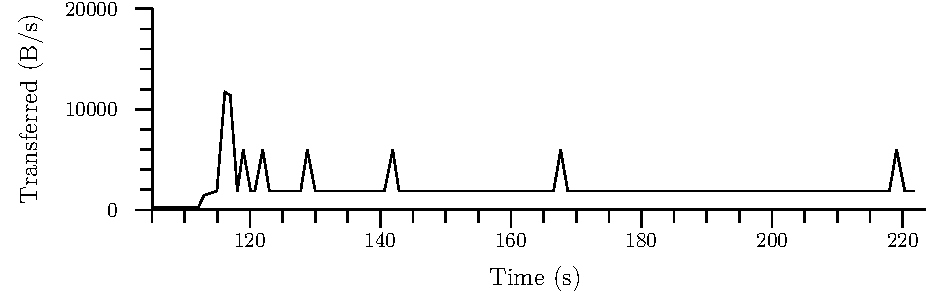
\includegraphics[width=1\textwidth]{diagrams/uIPFlowControl.pdf}
			\caption{Exponential back-off by computer when \uIP{} flow-control used}
			\label{fig:uIPFlowControl}
		\end{figure}
		
		By inspecting the packets sent and received, the window size is always
		obeyed but the packet announcing the window size becoming non-zero appears
		to be ignored. Wireshark's protocol checker did not report any errors and
		comparison with the known-working implementation in Linux did not reveal any
		fundamental differences. Unfortunately further study did not yield a
		diagnosis for the problem. Due to the time constraints imposed by the
		project TCP had to be dropped for G-code transmission in the project.
	
	
	\section{Temperature Readings}
		
		The temperature readings depended on correct values being read from the
		analog inputs and on correct calculation of the temperature based on these
		readings. Though consistency is important, reading temperatures close to the
		actual value is relatively unimportant as the temperature is fairly uneven
		within the heated components of the printer. The temperature values used
		during printing will be calibrated manually and the actual temperature in
		\dC{} is not significant but the consistency with which it is reached is.
		
		To test analog input, a selection of resistors with known values within the
		range of values the thermistor could exhibit were tested. As well as
		breadboard testing, the test was repeated on the final circuit board as the
		screw terminal used to connect the thermistors could also be used to connect
		a test resistor directly.
		
		When converted to a resistance using (\ref{equ:potdiv}), the values read
		were found to be within $\pm2\%$ of the resistor value as read by a
		multimeter (a difference which is accounted for by the fact that a second
		resistor with a $\pm5\%$ tolerance is used in the potential divider).
		
		To test that temperatures were being correctly converted from the resistance
		of the thermistors, an infra-red thermometer (figure \ref{fig:thermometer})
		was used to take temperature readings from the extruder and platform and
		these values were then compared against the value calculated using
		(\ref{equ:steinhart}). The heaters were turned on and readings were taken
		every minute as the extruder and platform heated up and then every five
		minutes for half an hour as it cooled down. The tests were repeated multiple
		times alongside other experiments, each time with similar results, to ensure
		consistency.
		
		The radius of the area measured by the thermometer becomes larger as it is
		moved further away from the target. Because the temperature across the
		platform and extruder vary greatly depending on location, the thermometer
		was placed close to the centre of the extruder nozzle and the centre of the
		build platform.
		
		\begin{figure}
			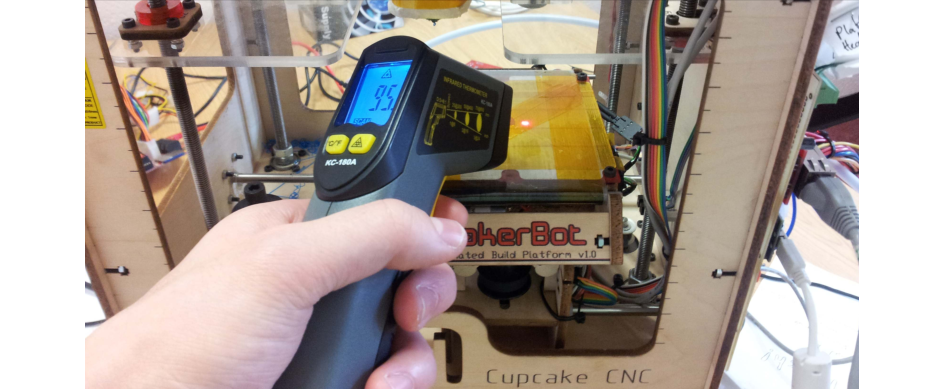
\includegraphics[width=1\textwidth]{diagrams/thermometer.pdf}
			\caption{Checking platform temperatures using an infra-red thermometer}
			\label{fig:thermometer}
		\end{figure}
		
		The temperatures recorded for the extruder were within $\pm1\dC$ below
		100\dC{} but rose to around $+8\pm1\dC$ around 220\dC{} (normal operating
		temperature).
		
		The platform temperatures were initially incorrect by $\pm10\dC$ or more.
		The platform contains a built in potential divider which was not used by the
		design (instead using the circuit on the main board) and was found to be
		connected to the main board. Once the connections were corrected, readings
		followed a similar pattern to the extruder (up to the 125\dC{} the platform
		is designed to operate at).
		
		The results above represent adequate performance for the task of maintaining
		a desired temperature and also show that the temperatures read are close to
		their real values such that an operator can safely tell from a temperature
		reading that the device is unsafe to touch.
	
	\section{PID Control}
		
		% XXX: Yeah...
		
		\label{sec:pidtraning}
		
		The PID controller has three constants ($K_p$, $K_i$ and $K_d$) which must
		be manually tuned to yield sensible system performance. While operating, the
		temperature oscillates around the set point. An optimal system has
		oscillations that are as small as possible and which responds as quickly as
		possible to changes in the set point or environment.
		
		PID controller tuning is a non-trivial problem for which automated solutions
		are either highly specialised or unavailable. Heuristics exist such as The
		Ziegler-Nichols method for selecting good values which work in many cases
		and require human interpretation \cite{ziegler}.
		
		% XXX: Jump?
		
		The Makerbot wiki suggests values (given in table \ref{tab:makerbotpid}) as
		a starting point requiring only a small amount of adjustment
		\cite{makerbotpid}. After selecting these values the printer's performance
		was monitored both while idle and during printing and the size of
		oscillations were measured. Performance was similar while in both states
		(with a temperature jump in platform temperature at the start of printing
		when molten plastic is extruded directly on to the platform). Oscillations
		were $\pm2\dC$ for the extruder and platform. Though this is greater than
		the $\pm1\dC$ recommended, print quality was not adversely effected.
		
		\begin{table}
			\centering
			\begin{tabular}{l l l}
				\toprule
				Constant & Extruder Value & Platform Value \\
				\midrule
				$K_p$    & $5.143$        & $7.0  $  \\
				$K_i$    & $0.0612$       & $0.342$ \\
				$K_d$    & $108.0$        & $36.0 $  \\
				\bottomrule
			\end{tabular}
			
			\caption{Generic PID controller constants for a Makerbot
			         \cite{makerbotpid}}
			\label{tab:makerbotpid}
		\end{table}
	
	\section{Stepper Control}
		
		The stepper control system consists of code for producing accurately timed
		steps and code for coherently moving the stepper motors. These two parts
		were tested separately as described in the following subsections. Finally,
		the results of these tests are evaluated.
		
		\subsection{Timing}
			
			To ensure timing accuracy, the three stepper signals were driven at a
			combination of frequencies with a frequency meter attached to the step
			pin. These tests were generated initially using a program on the
			microcontroller (so that the system was not under any load) and then using
			G-code sent over the network interface while other requests were being
			made (to place the system under reasonable load).
			
			The frequencies measured were exact to within the accuracy of the meter
			(four significant figures) for all tests.
			
			% XXX: What does that really mean?
			
		
		\subsection{Stepping}
			
			To test that stepping was happening coherently, with sequences of steps
			correctly spaced apart, the system was connected to the printer and
			circles were plotted on the axes. The circles are made up of short,
			continuous line segments where the relationship between the movements on
			each axis is not constant. Once again, the test was initially carried out
			using a test program running on the Mbed and then by G-code sent over the
			network. The number of segments the circle was divided into was increased
			from $30$ to $3,000$ and the speed set to $330\mm/\s$ and $3300\mm/\s$ to
			test slow and fast movements.
			
			The performance of the system was measured by visual inspection of the
			movement and circles plotted by attaching a pen to the extruder. The time
			taken the plot the circles was also measured using a timer on the Mbed to
			see if the overhead between each segment caused significant drift. Above
			around $100$ segments the circles drawn appeared smooth and at low and
			high speeds the overhead after 20 circles had been plotted at each speed
			and resolution was less than the $1\ms$ resolution of the timer. Finally,
			to ensure that steps were not being missed the system was homed to a known
			point between tests and this did not drift after all tests had completed.
			
		\subsection{Evaluation}
		
			The amount of plastic deposited at a given point during a print is
			dependent on the rate at which the plastic is extruded and also the rate
			at which the platform moves. The accuracy of the timing (combined with the
			mechanical properties of the machine) determines the platform's rate of
			movement. The print quality therefore depends on these factors.
			
			% XXX: Quantify
			
			The timing accuracy measured above indicates that errors caused by timing
			will be far smaller than the mechanical errors in the system. The
			inspection of the system actually stepping indicates that there is no
			significant timing drift caused by processing between movements. The tests
			also showed that the system can easily deal with plotting sub-millimetre
			paths.
	
	\section{End-stops}
		
		The endstops were tested under various lighting conditions to observe the
		effect on the opto-interrupters. The following lightings conditions were
		tested:
		\begin{itemize}
			\item Ambient strip lighting
			\item Ambient halogen lighting
			\item Ambient incandescent lighting
			\item Ambient natural light
			\item Direct halogen lighting
			\item Direct incandescent lighting
			\item Darkened room
		\end{itemize}
		
		Testing consisted of interrupting each opto-interrupter by moving the
		printer axes so that the end-stop should be triggered and observing the
		digital value read by the Mbed and the state of the debugging LED. Under all
		but the direct lighting conditions the correct value was read and the
		debugging LEDs were completely off or completely on. Under direct lighting,
		especially incandescent lighting, the state read by the Mbed for some
		end-stops was stuck where external light shone into the opto-interrupter. In
		these cases the debugging LEDs did not become completely `off' indicating
		that the opto-interrupter was being triggered.
		
		Though these results suggest that the end-stops cannot be used under direct
		lighting from halogen or incandescent bulbs, the system was found to perform
		well outside these conditions. Although not tested (due to unfavourable
		weather conditions), direct natural light may also have caused similar
		problems.
		
		% TODO: Moved to conclusions
		
		%To solve this problem, a more complex system can be implemented. The
		%infra-red LEDs in the opto-interrupters are pulsed by the microcontroller
		%and the photo-transistor's current is checked for the presence of these
		%pulses. External light sources are unlikely to contain the same pulses and
		%so the system can be sure of the origin of the light passing onto the
		%photo-transistor. Unfortunately this would require significant additions to
		%the electronics and a change to the end-stop interface. As a result, the
		%changes could not be made within the time frame of project. Instead the
		%printer should be used out of direct light to ensure that the end-stops
		%operate correctly.
	
	\section{Buffer Utilisation}
		
		To ensure that the printer did not stall during regular print jobs, the
		G-code and low-level command buffers were monitored during the execution of
		various test jobs. Buffer underruns or low buffer utilisation could indicate
		a performance issue in the G-code interpreter, network interface or their
		interaction with the operating system.
		
		The utilisation and size of each buffer along with a counter for the number
		of underruns experienced by the command-buffer are logged while various
		G-code files are sent to the printer. The test files consisted of:
		
		\begin{description}
			
			\item[Circle drawing with low detail] This test ensures that given a
			sequence of slow G-code instructions the printer keeps all buffers
			reasonably full and that the network interface can cope with infrequent
			small bursts of data.
			
			\item[Circle drawing with high detail] This test ensures that given a
			constant sequence of fast G-code instructions the printer keeps all
			buffers reasonably full and that no underruns occur during busy periods.
			
			\item[Circle drawing with high detail and pauses] This test ensures that
			given a sequence of fast G-code instructions separated by sleeps where the
			buffers filled and the network interface paused can quickly restart after
			the sleep.
			
			\item[Test box model] This non-synthetic test is a simple print job which
			contains long pauses (during heating and cleaning phases), relatively
			low-activity periods (border drawing) and reasonably detailed periods
			(fill patterns).
			
		\end{description}
		
		% TODO: Results
	
	\section{System Testing}
		
		The system was tested as a whole to assess its performance in both synthetic
		printing benchmarks and tests as well as printing real-world objects. These
		tests also aid in calibration of the G-code generator (Skeinforge). The
		synthetic tests allow the printer's performance to be objectively measured
		while real objects show real-world performance of the printer in its
		intended application.
		
		\subsection{Synthetic Tests}
			
			As a simple test of using all of the printer's components coherently, the
			circle plotting test was modified to produce spirals and the heaters and
			extruder enabled. Figure \label{fig:syntheticTests} shows samples of the
			output of these tests:
			\begin{description}
				
				\item[(A)] The extruder was moved at a safe distance from the platform
				to ensure that all components move together but without the risk of the
				extruder colliding with the platform or blocking the nozzle of the
				extruder.
				
				\item[(B)] As in (A) but the extruder is moved closer to the platform to
				test that the system can safely operate next to the platform and that
				the plastic adheres to the platform (and then properly detaches when
				ejected).
				
				\item[(C)] A larger spiral printed to test that the plastic adheres
				closer to the (colder) edges of the platform and that warping due to
				temperature changes during the print does not cause problems.
				
				\item[(D)] The winding of the spiral is tightened to test that the
				plastic adheres to itself and the platform and that warping does not
				cause the print to fail. Figure \ref{fig:looseSpiral} shows a print
				where the spiral was printed too loosely and it did not adhere to
				itself.
				
			\end{description}
			
			\begin{figure}
				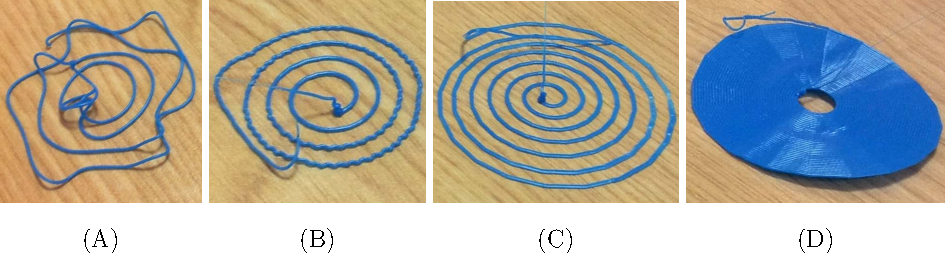
\includegraphics[width=1\textwidth]{diagrams/syntheticTests.pdf}
				\caption{Synthetic 3D printer tests for basic calibration}
				\label{fig:syntheticTests}
			\end{figure}
			
			\begin{figure}
				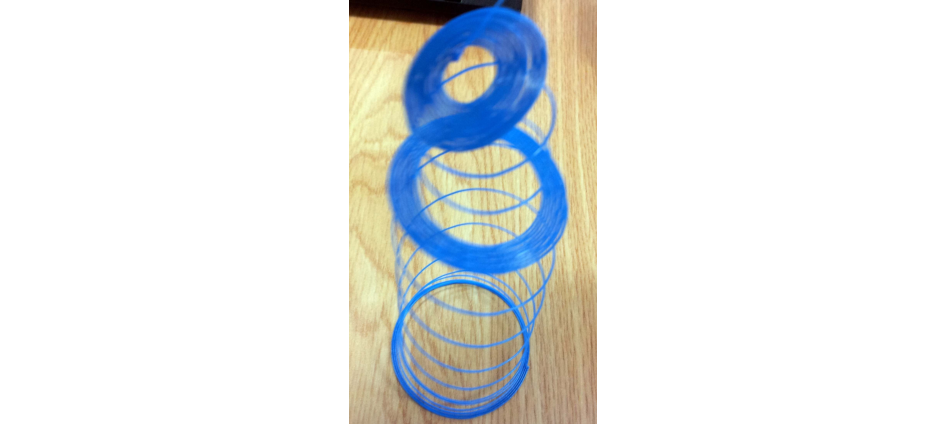
\includegraphics[width=1\textwidth]{diagrams/looseSpiral.pdf}
				\caption{Bad print of the test in figure \ref{fig:syntheticTests}(D)}
				\label{fig:looseSpiral}
			\end{figure}
			
			These prints were repeated, varying the platform temperature, Z-axis
			position (height) and the tightness of the spiral until the tests
			performed as described above. These tests ensure that the printer is
			capable of operating all its major components coherently in order to
			produce printed object.
			
			% TODO: Picture of Vernier caliper in use?
			
			% TODO: Actual cube measurements
			
			To test the system with G-code generated by Skeinforge, a simple 3D model
			of a cuboid (Figure \ref{fig:testCubes} (A)) was printed. This print
			yields a cuboid of known dimensions and is used to check calibration
			settings for Skeinforge. The cuboid is initially printed on top of a thick
			`raft' of plastic (used to ensure an even printing surface) and then
			separated using a chisel. The dimensions of the cuboid are then checked
			using a Vernier caliper to ensure that the printed object is of the
			correct size. The Makerbot wiki claims that $0.1\mm$ resolution is
			possible on a correctly tuned machine and so this requirement was used to
			judge prints \cite{makerbotfaq}.
			
			\begin{figure}
				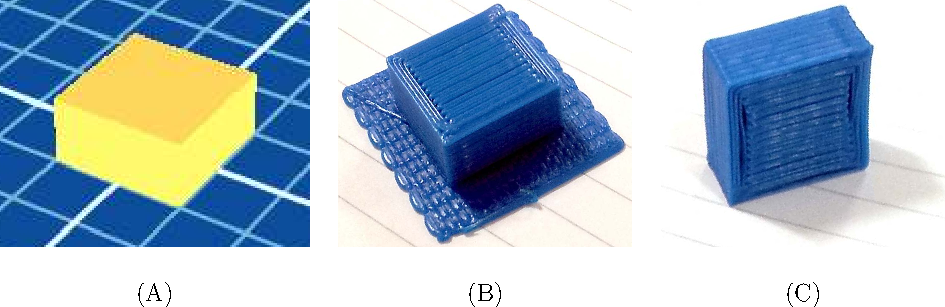
\includegraphics[width=1\textwidth]{diagrams/testCubes.pdf}
				\caption{Test cuboid model (A) print from Skeinforge G-code before raft
				         removal (B) and after raft removal (C)}
				\label{fig:testCubes}
			\end{figure}
			
		
		\subsection{Test Objects}
			
			To test the printer's ability to produce useful objects, various objects
			were printed including objects with moving parts and objects near the
			print-size limits for the printer. These tests check the system's ability
			to deal with large and complex loads. A large selection of printed test
			objects is provided in Appendix \ref{sec:examplePrints}.
			
			\subsubsection{Detailed Prints}
				
				Prints with detailed areas were used to test that the system could
				process the larger density of G-code at the required rate and also to
				ensure that steps were not missed during printing.
				
				For example, figure \ref{fig:vase} shows a vase which yields very short
				line segments while printing the corners of the shape. The previous
				electronics would not be able to process this design fast enough and
				would skip instructions causing steps to be missed. With the new
				electronics no buffer underruns or printing problems occurred during a
				run featuring a large version (shown) and a smaller version containing
				finer detail as a result.
				
				\begin{figure}
					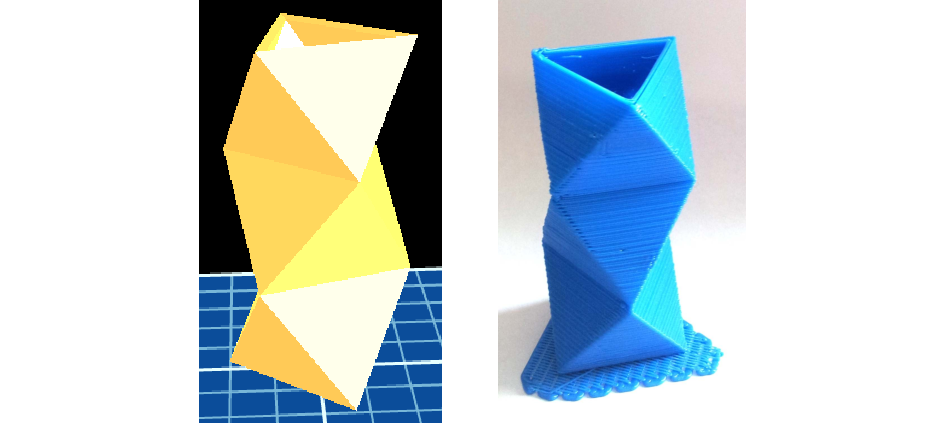
\includegraphics[width=1\textwidth]{diagrams/vase.pdf}
					\caption{3D printed vase with detailed corners}
					\label{fig:vase}
				\end{figure}
			
			\subsubsection{Large Prints}
				
				% XXX: No objective numbers...
				
				Large prints stress the printer and electronics for long periods and can
				reveal missed motor steps or instructions. The previous system had
				frequent issues printing large objects due to skipped instructions or
				steps and is a particular area for improvement.
				
				% TODO: Figure ref
				Of the large objects printed, only one failed to print. This was due to
				the object warping and becoming detached from the platform during the
				print causing the tip of the extruder to rip the object off the platform
				(figure \ref{fig:}). Unevenness in the temperature of the object during
				printing is the cause of this distortion. This is partially caused by
				unevenness in the temperature of the build platform. Unfortunately, this
				is a problem with the printer's design which is not addressed in this
				project.
				
				% TODO: Picture of damaged large print
				
				% XXX: Conclude...?
			
			\subsubsection{Raftless Printing}
				
				Though the first prints were completed on top of a raft, it was later
				disabled. This reduced print time, improved print quality and allowed
				intricate designs such as a comb to be printed (figure \ref{fig:comb})
				where removal of the raft would damage the design.
				
				\begin{figure}
					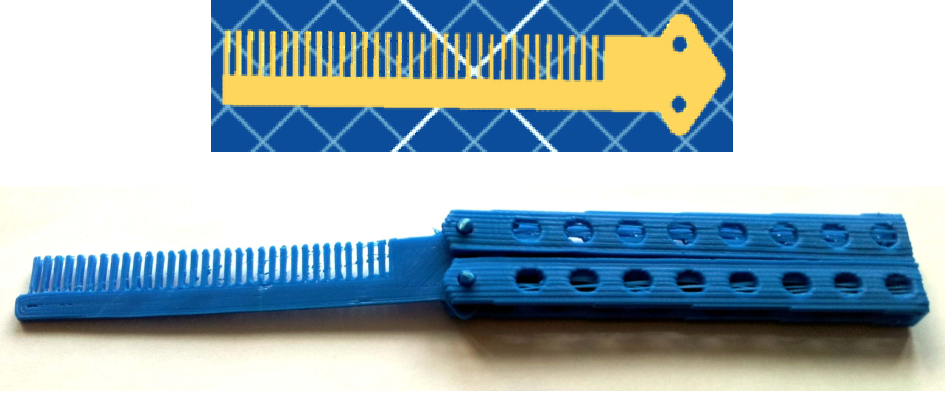
\includegraphics[width=1\textwidth]{diagrams/comb.pdf}
					\caption{Folding `butterfly comb', printed without a raft (designed by
					         techno246 \cite{butterflycomb})}
					\label{fig:comb}
				\end{figure}
				
				Many objects were reprinted using raftless printing and performance was
				generally similar with the exception of larger designs. These
				experienced greater warping without the support of the raft and thus
				were more prone to failure due to the extruder hitting the object.
				
				% XXX: Conclude
